\documentclass[a4paper, draftcls]{IEEEtran} % onecolumn
%
\usepackage{subscript}
\usepackage[T1]{fontenc}
\usepackage[utf8]{inputenc}
\usepackage{amssymb}
\usepackage{graphicx}
\usepackage{tikz}
\usepackage{fancybox}
\usepackage{algorithm}
\usepackage{algorithmic}
\usepackage{listings}

\usepackage{pgf}
\usepackage{tikz}
\usetikzlibrary{arrows,automata}




\begin{document}


\title{ Report f\"ur SOS}

\author{
  \IEEEauthorblockN{Robert Oehlmann, Jan Winkelmann}
  \IEEEauthorblockA{\\Hamburg University of Technology\\
    Institute of Communication Networks\\
  }
}

\maketitle

%\begin{abstract}
%  \boldmath
%  \input{abstract}
%\\end{abstract}

\IEEEpeerreviewmaketitle
\IEEEoverridecommandlockouts

\section{Einleitung} \label{sec:intro}
Robert und jan schreiben hier \"uber die einleitung

\section{Setting} \label{sec:setting}
Dieser Abschnitt beschreibt zuerst das Anwendungsgebiet, und danach die Annahmen die bei dem Design des Protokolles gemacht wurden.
W\"ahrend des Entwerfens des Protokolles, wurde nicht drauf geachtet das Anwendungszenario realistisch zu gestalten. Weder das Anwendungsszenarion noch Annahmen beruhen auf recherchierten Fakten.

\subsection{Anwendungsgebiet}
Um Fr\"uhwarnsysteme f\"ur Waldbr\"ande zu verbessern k\"onnten z.B. kleine Sensoren eingesetzt werden, welche sich untereinander vernetzen um so gro\ss e Fl\"achen messen zu k\"onnen.
In unserem Szenario seien Sensoren gegeben, die neben dem Messen von Metriken die f\"ur die Waldbranderkennung n\"otig sind, auch \"uber zwei Kommunikationsmethoden verf\"ugen. Eine Kommunikationsm\"oglichkeit zur Verst\"andigung mit anderen Sensoren in der unmittelbaren Umgebung, wie zum Beispiel W-LAN, und eine zum Senden der Messergebnisse an eine Senke, wie zum Beispiel GPRS.

Ziel dieses Projektes es nun, Sensorknoten in \emph{Cluster} zu organisieren.
Cluster benuzten Kurzstrecken-Kommunikation um den Sensoren zu erm\"oglichen Energie zu sparen, indem die Messdaten bei manchen Sensoren gesammelt werden, und so nicht jeder Sensor seine Daten einzeln zu der Senke senden muss.
Die Sensoren, welche die Messdaten zur Senke sendet bezeichnen wir als \emph{Clusterhead}.

\subsection{Annahmen}
Die technischen Voraussetzungen f\"ur unseren Ansatz sind die Folgenden:
\begin{itemize}
\item Alle Sensorknoten sind baugleich, d.h. jeder Sensorknoten kann mit anderen Sensorknoten und der Senke kommunizieren.
\item Keine zwei Sensorknoten versuchen gleichzeitig einem Cluster beizutreten. Dies wird  dadurch erreicht, dass alle  Sensorknoten sich nacheinander aktivieren.
\item Sensorknoten bewegen sich nicht.
\item Keine Ausfälle von einzelnen Verbindungen. Ein Sensorknoten erreicht entweder alle Knoten seines Clusters, oder keine.
\item Keine tempor\"aren Ausf\"alle. Ein Sensorknoten f\"allt entweder nicht oder komplett aus.
\item Wenn ein Sensorknoten ausf\"allt, so merken es alle Sensorknoten im Cluster gleichzeitig und mit Sicherheit, aber nicht zwingend instantan.
\end{itemize}

\noindent Zus\"atzlich nehmen wir an, dass ein unterliegendes Protokoll existiert, das folgendes garantiert:
\begin{itemize}
\item Garantierte Zustellung von Nachrichten
\item Zustellung der Nachrichten in der richtigen Reihenfolge
\end{itemize}
Ein Beispiel hierf\"ur w\"are ein TCP/IP Stack.

\section{Funktionale Anforderungen} \label{sec:features}
\begin{enumerate}
\item \textbf{Implementation des beschriebenen Protokoll}
  \begin{itemize}
  \item \emph{Beschreibung:}\\
    Das Protokoll bietet die Hauptfunktionalit\"at f\"ur das Anwendungszenario. Eine vollst\"andige und fehlerfreie Implementation ist daher \emph{kritisch}.
  %\item \emph{Problembeschreibung:}\\

  \item \emph{Siehe:}\\
    Abschnitt \ref{sec:algo} f\"ur die Spezifikation des Protokolls.
  \item \emph{Abnahmekriterium:}\\
    Dierse Anforderung gelte als erf\"ullt, wenn die Implementation folgendes leistet: das Bilden von Verb\"unden, das Behandeln von Ausf\"allen von Sensorknoten und die Rotation von Verbundsleitern anhand des genannten Protokolls.
  \end{itemize}

\item \textbf{Kapselung der Komponenten}
  \begin{itemize}
  \item \emph{Beschreibung:}\\
    Einzelne Systemkomponenten haben auf realistische Weise voneinander gekapselt sein.
    Dies bezieht sich insbesondere, aber nicht aussschlie\ss lich auf den Motes zur Verf\"ugung stehenden Informationen, wie Lage, Informationen \"uber andere Sensorknoten, sowie Zustellung der Kommunikationen unter dem Motes durch einen von dem Sensorknoten unabh\"anigen Mechanismus.
  \item \emph{Problembeschreibung:}\\
Um eine m\"oglichst realistische Simulation zu sein, und um als echter Proof-Of-Concept zu gelten, m\"ussen die simulierten Komponenten voneinander entkoppelt sein, also \"uber Schnittstellen kommunizieren, welche auch in einem Anwendungszenarion bestehen w\"urden.
  \item \emph{Abnahmekriterium:}\\
    Zur Erf\"ullung dieser Anforderung sind n\"otig: Kapselung der Mote-Objekte untereinander, Kapselung der Mote-Objekte von der Simulationsumgebung und ein Mechanismus zum Nachrichtenversenden.
  \end{itemize}
\item \textbf{Graphische Oberfl\"ache}
  \begin{itemize}
  \item \emph{Beschreibung:}\\
    Die Implementation hat eine graphische Benuzteroberfl\"ache zur Verf\"ugung zu stellen, welche die Simulation visualisiert. Die Bedienung der Oberfl\"ache hat ein sinnvolles Subset der Gesamtfunkionalit\"at zu implementieren.
  \item \emph{Problembeschreibung:}\\
    Um die Simulation zu visualisieren ist eine graphische Oberfl\"ache unentbehrlich. Sie dient zur demonstration des Proof-Of-Concepts. Das Hinzuf\"ugen und Entfernen von Motes erlaubt das Demonstrieren des vollen Umfanges der Funktionalit\"at.
  \item \emph{Abnahmekriterium:}\\
    Die Implementation muss eine graphische Benuzteroberfl\"ache haben, welche die simulierte Umgebung, samt Sensoreknoten darstellt. Gebildete Cluster m\"ussen farblich markiert sein. Zus\"atzlich soll man Sensorknoten hinzuf\"ugen und entfernen k\"onnen.
  \end{itemize}
\end{enumerate}

\section{Algorithmen}
Dieser Abschnitt besch\"aftigt sich mit den entwickelten Algorithmen f\"ur das bilden von Clustern, die Ausfallsicherheit, und das Rotieren von Clusterheads.

\subsection{Clusterbildung}
Die Grundlage des Clusteringalgorithmus ist das Bilden von vollst\"andigen Graphen.
Die Knoten des Graphen sind die Sensoren, und die Kanten die W-Lan Verbindungen in Reichweite.
Dadurch reduziert sich die Clusterbildung auf das Cliquenproblem.

Cluster werden durch folgendes Protokol gebildet:
\begin{itemize}
\item Falls sich ein Sensor aktiviert, so sendet sie zuerst eine Nachricht die nach vorhandenen Clustern sucht. Findest der Sensor keine vorhandenen Cluster, so bildet er selber einen.
\item Alle schon vorhandenen Clusterheads antworten auf die Anfragen von neuen Motes. Diese Antwort enth\"allt einen Identifikator des Clusters und die Anzahl der Sensoren in dem Cluster.
\item Der neue Sensor speichert alle Antworten der vorhanden Cluster, ordnet sie nach Gr\"o\ss e und versucht der Reihe nach einem der Cluster beizutreten, beginnend mit dem Kleinsten.
\item Der erste Schritt zum Beitreten eines Clusters, das Senden eine Nachricht, auf die alle Mitglieder des Clusters mit ihrer Id antworten.
\item Nach dem Ablaufen eines Timeouts, sendet der neue Sensor die Ids aller empfangenen Sensoren an den Clusterhead. Dies stellt sicher, dass der neue Sensor alle schon vorhandenen Mitglieder erreichen kann.
\item Falls die Nachricht des neuen Sensors alle Ids des aktuellen Clusters entahlten, so sendet der Clusterhead dem neuen Sensor eine Nachricht mit der Best\"atigung, dass er neue Sensor dem Cluster beigetreten ist. Zus\"atzlich ordnet der Clusterhead dem neuen Sensor einen Slot zu. Dieser Slot wird n\"otig, falls der Clusterhead ausf\"allt.
\item Falls die Nachricht des neuen Sensors nicht alle Ids enthalten sollte, so sendet der Server eine Ablehnung und der Client versucht dem n\"achst gr\"o\ss eren Cluster beizutreten.
\end{itemize}

\begin{figure}
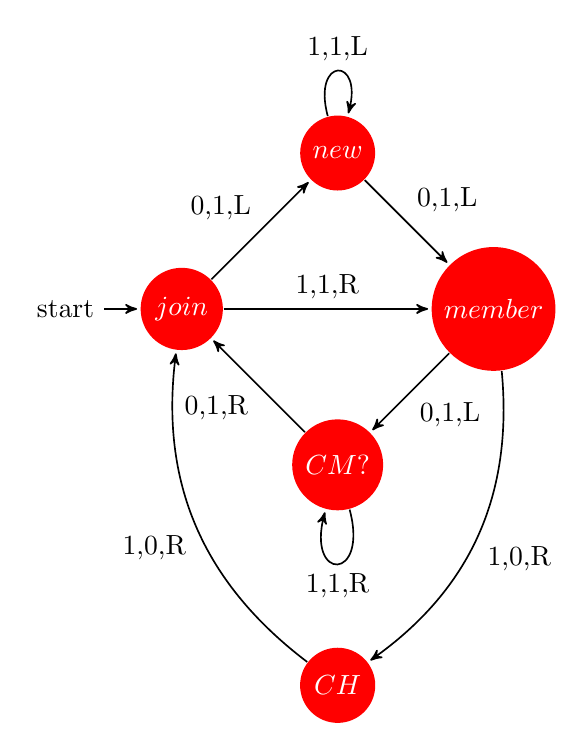
\begin{tikzpicture}[->,>=stealth',shorten >=1pt,auto,node distance=2.8cm,
                    semithick]
  \tikzstyle{every state}=[fill=red,draw=none,text=white]

  \node[initial,state] (A)                    {$join$};
  \node[state]         (B) [above right of=A] {$new$};
  \node[state]         (D) [below right of=A] {$CM?$};
  \node[state]         (C) [below right of=B] {$member$};
  \node[state]         (E) [below of=D]       {$CH$};

  \path (A) edge              node {0,1,L} (B)
            edge              node {1,1,R} (C)
        (B) edge [loop above] node {1,1,L} (B)
            edge              node {0,1,L} (C)
        (C) edge              node {0,1,L} (D)
            edge [bend left]  node {1,0,R} (E)
        (D) edge [loop below] node {1,1,R} (D)
            edge              node {0,1,R} (A)
        (E) edge [bend left]  node {1,0,R} (A);
\end{tikzpicture}
\ref{fig:sm}
\caption{State Machine des Cluster Protokolls}
\end{figure}
\subsection{Ausfallsicherheit} \textbf{TODO}
Aufgrund der erw\"ahnten Annahmen (TCP/IP, keine Bewegung der Motes, etc) gibt es nur zwei Ausfallszenarien die betrachtet werden m\"ussen, der Ausfall einer Membermote,  sowie der Ausfall des Clusterheads.
Falls eine Membermote ausfallen sollte, so muss der zugeh\"orige Clusterhead dies merken und die Liste der zum Cluster zugeh\"origen Motes aktualisieren.
Da Motes die dem Cluster betreten wollen Kontakt zu allen Motes nachweisen m\"ussen, die der Cluster als zum Cluster zugeh\"orig gespeichert hat, w\"urde der unbemerkte Ausfall einer Mote dazu f\"uhren, dass keine neuen Motes beitreten k\"onnen.
In einem realen Szenario erkennt der Clusterhead das Ausfallen einer Membermote an dem Fehler von gesendeten Sensordaten. In der nie vorgestellten Simulation wird durch das L\"oschen direkt beim Server ein L\"oschevent.

Der Ausfall von einem Clusterhead wird durch das Fehlen von Best\"atigungsnachrichten erkannt.
Aufgrund unserer Annahme geschickt dies bei allen Membermotes gleichzeitig.
Sobald eine Membermote den Ausfall des Clusterheads wahrnimmt, so wird der Cluster als tot angenommen.
Die Mote wartet nun eine bestimmte Zeit $b$ und versucht dann einem neuen Cluster beizutreten.
$b$ berechnet sich durch die upper bound f\"ur das Beitreten einer Mote zu einem Cluster multipliziert mit dem ``slot'' welcher der Mote beim Beitreten des jetzt toten Clusters zugewiesen wurde.
Der slot ist ein streng monoton ansteigender pro Cluster eindeutiger Integer.
Somit wird sichergestellt, dass die Membermote alle nacheinander in der urspr\"unglichen Beitrittsreihenfolge versuchen einem neuen Cluster beizutreten.

\subsection{Rotation der Clusterheads} \textbf{TODO}
Die Rotation des Clusterhead ist der Prozess welcher von dem aktuellen Clusterhead ausgef\"uhrt wird, und einer Membermote die F\"uhrung des Clusters zuweist.
Dieser Rotation kann ausgel\"ost werden von z.B. einem timeout oder dem Batteriestand.
Beider Durchf\"uhrung der Rotation w\"ahlst der Clusterhead der neuen Cluster und sickt alle relevanten Daten an ihn.
Die gesendeten Daten sind:
slot\\
Membermotes\\
...\\

\section{Implementierung} \label{sec:impl}

Um die dargelegten Algorithmen zu testen und zu demonstrieren, haben wir
eine Simulation entwickelt. Im folgenden wird zunächst die gewählte
Entwicklungsplattform vorgestellt und begründet, anschließend werden die
Implementierung des Äthers, der Sensorknoten und die Spezifika der
Simulations-Umgebung dargestellt.

\subsection{JavaScript}

Die Simulation ist in JavaScript implementiert; als
Entwicklungsplattform haben wir Webbrowser mit aktueller
JavaScript-Engine (z.B. Googles V8 und Mozillas JägerMonkey) und
Unterstützung für 2D-Grafikdarstellung mithilfe des canvas-Tags gewählt.

Mit JavaScript als dynamisch typisierter, prototypenbasierter
Skriptsprache lassen sich ohne große Deklarations-Overhead schnell
sichtbare Ergebnisse produzieren. Mit dem neuen HTML5 Canvas Element
steht eine einfach zu nutzende Zeichenfläche zur Verfügung und für alle
gängigem Betriebssysteme gibt es Browser die die Simulation auführen
können.

Obwohl JavaScript eine klassenlose Sprache ist, werde ich ähnliche
Termini wie in anderen objektorientierten Sprachen (also auch den
Terminus ``Klasse'') verwenden.

\subsection{Sensorknoten}

Die simulierten Sensorknoten sind Instanze der Klasse ``Mote'', deren
Implementierung sich über die Dateien mote.js, mote\_member.js und
mote\_head.js erstreckt.

Das in Abschnitt \ref{sec:algo} dargestellte Protokoll ist vollständig, aber
zustandslos, in der Klasse Mote implememtiert.

Wird ein neuer simulierter Sensorknote von der Klasse Mote instanziiert,
initialisiert der Konstruktur einige interne Variablen und registriert
den neuen Sensorknoten beim Äther; anschließend kann dieser gestartet
(``eingeschaltet'') werden.

\subsection{Äther}

Die simulierten Sensorknoten kommunizieren untereinander nur über
Nachrichten. Den (virtuellen) Versandt der Nachrichten übernimmt der
simulierte Äther, implementiert als Modul
\footnote{\url{http://yuiblog.com/blog/2007/06/12/module-pattern/}} ``MoteList'' in der
Datei motelist.js.

Ähnlich dem Observer-Entwurfsmuster stellt MoteList eine Methode
``register'' bereit, die neuer Sensorknoten aufnimmt. Sie wird vom
Mote-Konstruktur aufgerufen. Zudem gibt es eine Methode ``send'', die
den Versandt von Nachrichten anstößt.

Beim Versandt wird zunächst die Position des Absenders abgerufen,
anschließend wird die Distanz zu allen anderen registrierten
Sensorknoten berechnet. Ist die Distanz nicht größer als ein
festgelegter Senderadius, wird die Nachricht zugestellt indem sie der
``onRecv'' Methode des jeweiligen Empfänger-Knotens übergeben wird. Der
Absender erhält seine eigenen Nachrichten nicht.

\subsection{Nachrichten}

Bei den übergebene Nachrichten handelt es sich um JavaScript-Objekte.
Sie sind nicht Instanzen einer bestimmten Klasse sondern nur des
Basis-Typs Object, somit folgen sie auch keinem strikten Format.

Alle Nachrichten haben jedoch per Konvention eine Eigenschaft ``type'',
die Aufschluss über die Intention der Nachricht gibt (z.B. WHOISTHERE,
JOINREQ, ROTATE) und somit auch die Kodierung der übrigen Eigenschaften
impliziert.

Über eine Netzwerk könnten die Nachrichten JSON-kodiert verschickt
werden, in der Simulation verzichten wir jedoch zugunsten der
Performance auf das Marshalling und Unmarshalling beim Absender
respektive Empfänger.

\subsection{Zeit}

Um die Geschwindigkeit der Simulation regulieren zu können sind alle
relevanten Zeitfenster (also insbesondere Timeouts) an die globale
Variable timeScale gekoppelt.

\subsection{Grafische Oberfläche}

Die grafische Oberfläche beschränkt sich im wesentlichen auf eine
``Karte'' in der alle Motes, möglichen Verbindungen, sowie Cluster
verzeichnet sind.

Die Zeichenfunktion ist dabei im Modul MoteList implementiert, da nur
darin Zugriff auf die Positionen der Sensorknoten möglich ist.

Die Sensorknoten sind als kleine Quadrate auf der Karte dargestellt,
oberhalb eines Cluserheads wird jeweils die ID des Clusters angezeigt.
Zwischen Sensorknoten die nicht mehr als einen Senderadius voneinander
entfernt sind, ist eine blasse Linie eingezeichnet. Zwischen zwei Knoten
die zu einem Cluster gehören, wird diese Linie farblich hervorgehoben.

Weitere Sensorknoten werden hinzugefügt, wenn man auf eine freie Fläche
der Karte klickt. Klickt man einen vorhandenen Knoten an, wird dieser
entfernt.

Die Rotation der Cluster-Heads wird durch Drücken der Taste 'r'
angestoßen. Die Taste 'a' schaltet die automatische Rotation der
Cluster-Heads in einem fixen Intervall ein oder aus.

\section{Analyse} \label{sec:ana}

Im folgenden wollen wir überprüfen, ob die Implementierung die in
Abschnitt III formulierten Anforderungen erfüllt und die Performance der
Simularion untersuchen.

\subsection{Implementierung des Protokolls}

Die Bildung von Clustern ist in den simulierte Sensorknoten gemäß der
Spezifikation in Abschnitt \ref{sec:algo} implementiert. In der Simulation können
Sensorknoten sowohl automatisch, als auch manuell platziert werden und
die Knoten schließt sich dann zuverlässig einem Cluster an oder eröffnen
ein neues.

Entsprechend der Spezifikationen erkennen Sensorknoten das Verschwinden
anderer Knoten nicht selber, reagieren aber wie im Protokoll festgelegt,
sobald sie über den Ausfall informiert werden.

Die Rotation des Clusterheads erfolgt bei Clustern mit mehreren Knoten
ebenfalls nach Protokoll, jedoch wird (entsprechend der Spezifikation)
nur nach externem Impuls rotiert und die Funktion des Clusterheads
übernimmt ein zufällig ausgewählter, anderer Sensorknoten.

\subsection{Kapselung der Komponenten}

Eine grundlegende Kapselung der simulierten Sensorknoten untereinander
besteht bereits darin, dass die Knoten jeweils als Instanzen der Klasse
Mote realisiert sind.

Referenzen auf die Sensorknoten (also die Instanzen der Klasse Mote)
werden nur innerhalb des MoteList Modules gespeichert. Die Liste der
Sensorknoten ist im Modul-Entwurfsmuster der MoteList durch den
Variablen-Skopus geschützt und nur Funktionen dieses Moduls können
darauf zugreifen. Der direkte Zugriff zwischen Sensorknoten ist somit
per Design ausgeschlossen.

Zusammen mit der Liste der Sensorknoten werden auch die Positionen der
Knoten im Modul MoteList geschützt gespeichert. Damit sind alle
relevanten Informationen der Simulationsumgebung vor den Sensorknoten
abgekapselt.

Die Kommunikation der Sensorknoten untereinander läuft somit
ausschließlich über den Nachrichtenversand, der im Äther (Modul
MoteList) implementiert ist. Nachrichten werden unter Berücksichtigung
eines Senderadius nur an ein Subset aller Sensorknoten übermittelt.

\subsection{Graphische Oberfläche}

Wie in den funktionalen Anforderungen gefordert, wird in der
Kartenansicht die simulierte Umgebung mit den darin enthaltenen
Sensorknoten dargestellt. Cluster werden durch farbige Linien zwischen
allen Knoten des Clusters als zusammenhängende Einheit erkennbar
gemacht.

Sensorknoten können hinzugefügt und entfernt werden.

\subsection{Performance}

Eine gute Performance war nicht Ziel dieser Simulation und ist im
Ergebnis auch nur für Demonstrationszwecke ausreichend.

Probleme treten auf, wenn die Nachrichten-Verteilung nicht schnell genug
erfolgen kann und Timeouts der Sensorknoten ablaufen, bevor die
Nachrichten zugestellt wurden. Das führt meistens dazu, dass
Sensorknoten nicht von vorhandenen Clustern erfahren oder nicht
rechtzeitig alle Mitglieder eines Clusters auflisten können, somit der
Beitritt zu vorhanden Clustern fehlschlägt und unnötig neue Cluster
gegründet werden.

Wie viele Sensorknoten ohne verspätete Zustellung von Nachtichten
bewältigen kann, hängt stark von der gewählten
Simulationsgeschwindigkeit, sowie der der verwendeten JavaScript-Engine
und natürlich der Rechenleistung eines CPU-Kerns ab. Ebenso beeinflusst
die Verteilung der Sensorknoten und der Senderadius die Performance:
Liegen die Sensorknoten stark geballt oder ist der Senderadius groß
gewählt, werden alle Nachrichten von vielen Knoten empfangen und das
System kommt schneller an seine Grenzen, als bei weit verteilten
Sensorknoten und kleinen Senderadien.

Bei den Standardeinstellungen (Karte mit 780x1248 Positionen,
Senderadius von 15\% der Kartenhöhe, 150 Sensorknoten) werden alleine
800 Nachrichten verschickt und rund 3000 bis 3300 Nachrichten empfangen.

Platziert man dagegen nur 30 Knoten so dicht beieinander, dass sie ein
einzelnes Cluster bilden, werden dabei bereits 551 Nachrichten
verschickt und 10.294 Nachrichten empfangen. Zwingt man dieses Cluster
zur Neubildung, indem man den Clusterhead löscht, entstehen dabei
innerhalb von 5 Sekunden nochmal 519 Nachrichten die 14.533 mal
empfangen werden.

Die obenstehenden Versuche wurden auf einem Core2Duo Mobil-Prozessor mit
1,87GHz Kerngeschwindigkeit in Googles Browser Chrome mit der
V8-JavaScript-Engine durchgeführt. Während der Clusterneubildung wurde
ein Prozessorkern für 5 Sekunden voll ausgelastet.

Aufgrund der vielen Faktoren die die Performance beeinflussen soll hier
auf eine weitere Analyse der Performance auf verschiedenen Systemem
verzichtet werden.

Mit den Standardeinstellungen und in einem aktuellen Browser sollte es
problemlos möglich sein, die Simulation zu testen.

\section{Analyse}
Robert... (This is also a placeholder)



\section{Future Work}
Jan will write about future work here.


\end{document}
